\documentclass[tikz,border=0pt]{standalone}
\usepackage{fontspec}
\usepackage{amsmath}
\usetikzlibrary{arrows.meta}

\setmainfont{Noto Sans CJK TC}
\setsansfont{Noto Sans CJK TC}

\newif\ifdarkmode
\ifdefined\darkmodeflag
  \darkmodetrue
\fi

\ifdarkmode
  \definecolor{pagebg}{HTML}{0B1120}
  \definecolor{textfg}{HTML}{E5E7EB}
  \definecolor{mutedfg}{HTML}{9AA7B8}
  \definecolor{edge}{HTML}{CBD5E1}
  \definecolor{thin}{HTML}{334155}
  \definecolor{panel}{HTML}{111827}
  \definecolor{panelborder}{HTML}{334155}
  \definecolor{accent}{HTML}{60A5FA}
\else
  \definecolor{pagebg}{HTML}{FFFFFF}
  \definecolor{textfg}{HTML}{172033}
  \definecolor{mutedfg}{HTML}{64748B}
  \definecolor{edge}{HTML}{334155}
  \definecolor{thin}{HTML}{D7DEE8}
  \definecolor{panel}{HTML}{F8FAFC}
  \definecolor{panelborder}{HTML}{D7DEE8}
  \definecolor{accent}{HTML}{2563EB}
\fi

\newcommand{\panel}[5]{%
  \begin{scope}[shift={(#1,#2)}]
    \draw[fill=panel, draw=panelborder, line width=0.7pt, rounded corners=4pt]
      (0,0) rectangle (4.65,5.35);
    \node[anchor=west, text=textfg, font=\sffamily\bfseries] at (0.32,4.92) {#3};
    \begin{scope}[shift={(2.35,2.35)}, scale=#4]
      \clip (-2.9,-2.05) rectangle (2.25,2.05);
      \draw[edge, line width=0.85pt] (-2.9,0) -- (2.25,0);
      \draw[edge, line width=0.85pt] (0,-2.05) -- (0,2.05);
      #5
      \fill[edge] (0,0) circle (2.2pt);
      \node[text=textfg, anchor=south west, font=\sffamily\fontsize{8}{10}\selectfont] at (0.05,0.05) {$F$};
    \end{scope}
  \end{scope}
}

\begin{document}
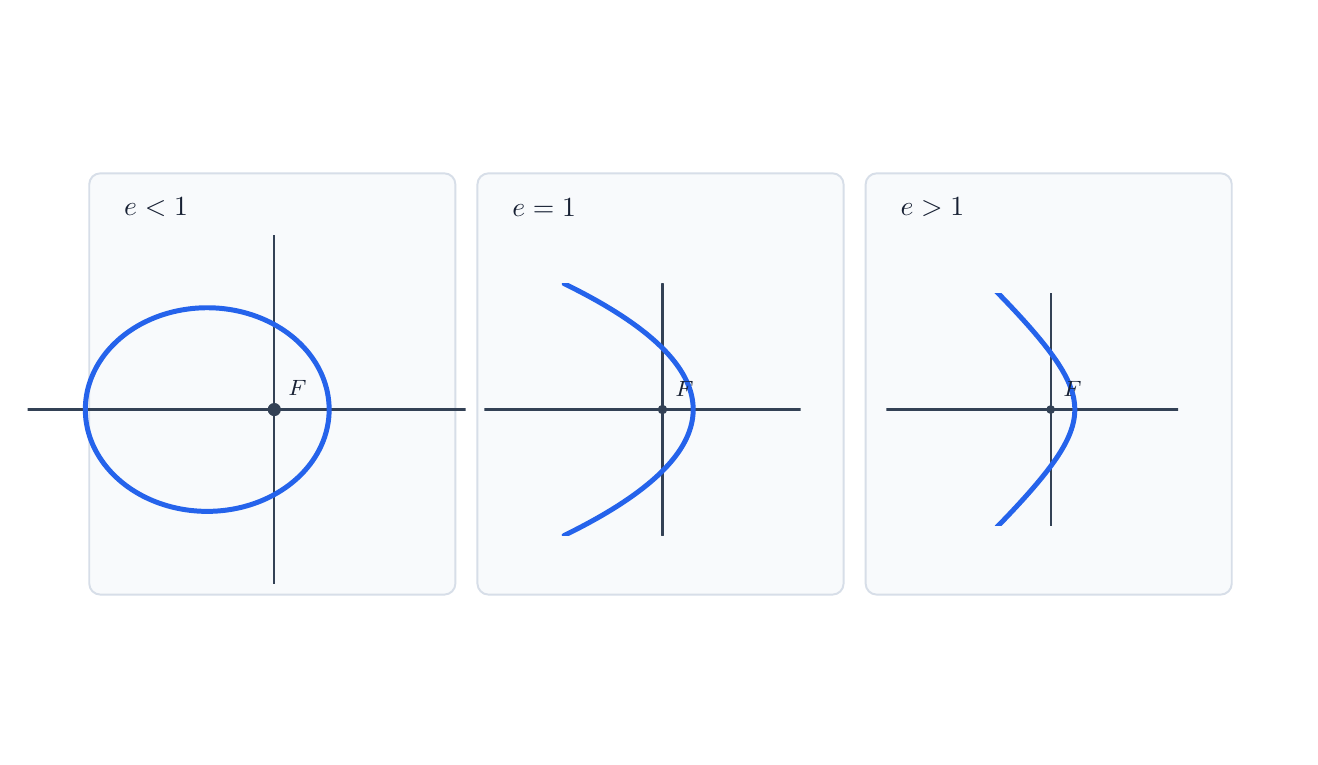
\begin{tikzpicture}[
  x=1cm,
  y=1cm,
  font=\sffamily,
  line cap=round,
  line join=round,
  >=Latex
]
  \fill[pagebg] (0,0) rectangle (16,9);

  \panel{0.75}{1.8}{$e<1$}{1.08}{
    \draw[accent, line width=1.8pt, smooth, variable=\t, domain=-180:180, samples=240]
      plot ({(1/(1+0.55*cos(\t)))*cos(\t)}, {(1/(1+0.55*cos(\t)))*sin(\t)});
  }

  \panel{5.68}{1.8}{$e=1$}{0.78}{
    \draw[accent, line width=1.8pt, smooth, variable=\t, domain=-128:128, samples=240]
      plot ({(1/(1+cos(\t)))*cos(\t)}, {(1/(1+cos(\t)))*sin(\t)});
  }

  \panel{10.61}{1.8}{$e>1$}{0.72}{
    \draw[accent, line width=1.8pt, smooth, variable=\t, domain=-123:123, samples=260]
      plot ({(1/(1+1.35*cos(\t)))*cos(\t)}, {(1/(1+1.35*cos(\t)))*sin(\t)});
  }
\end{tikzpicture}
\end{document}
